\documentclass[paperwidth=40in,paperheight=32in,landscape]{baposter} % Set poster size and orientation

\usepackage{amsmath,amssymb}
\usepackage{graphics}
\graphicspath{{images/}}
\usepackage{color}
\usepackage{multicol}
	\setlength{\columnseprule}{1pt}
	\def\columnseprulecolor{\color{black}}

\usepackage{enumitem}
	
\newcommand{\headshotsize}{0.95in}
% \newcommand{\headshotsize}{1.0in}
%%% Color Definitions %%%

\definecolor{cuGold}{cmyk}{0, .10, .48, .22}
\definecolor{cuBlack}{cmyk}{0, 0, 0, 1.00}
\definecolor{cuDarkGray}{cmyk}{.38, .28, .21, .63}
\definecolor{cuLightGray}{cmyk}{.16, .11, .11, .29}

\definecolor{bordercol}{RGB}{0,0,0} % Content cell border color
\definecolor{headercol}{RGB}{229,240,241} % Concent cell header fill color
\definecolor{headerfontcol}{RGB}{0,0,0} % Concent cell header text color
\definecolor{boxcol}{RGB}{255,255,255} % Concent cell background color

% Custom commands
\newcommand{\RR}{\mathbb{R}}
\newcommand{\NN}{\mathbb{N}}
\newcommand{\OO}{\mathcal{O}}
\newcommand{\mathcow}{\OO}
\newcommand{\QQ}{\mathbb{Q}}
\newcommand{\ZZ}{\mathbb{Z}}
\newcommand{\CC}{\mathbb{C}}
\newcommand{\KK}{\mathbb{K}}
\newcommand{\PP}{\mathcal{P}}
\newcommand{\TT}{\mathcal{T}}
\newcommand{\BB}{\mathcal{B}}
\newcommand{\LL}{\mathcal{L}}
\renewcommand{\Re}{\operatorname{Re}}
\renewcommand{\Im}{\operatorname{Im}}

\newcommand{\veca}{\vec{a}}
\newcommand{\vecb}{\vec{b}}
\newcommand{\vecd}{\vec{d}}
\newcommand{\vece}{\vec{e}}
\newcommand{\vecf}{\vec{f}}
\newcommand{\vecn}{\vec{n}}
\newcommand{\vecp}{\vec{p}}
\newcommand{\vecr}{\vec{r}}
\newcommand{\vecu}{\vec{u}}
\newcommand{\vecv}{\vec{v}}
\newcommand{\vecw}{\vec{w}}
\newcommand{\vecx}{\vec{x}}
\newcommand{\vecy}{\vec{y}}
\newcommand{\vecz}{\vec{z}}

\renewcommand{\vec}[1]{\mathbf{#1}}
\newcommand{\norm}[1]{\left\lVert #1 \right\rVert}

%%% Document Start %%%

\begin{document}

%%% Poster Settings %%%

\begin{poster}{
	grid = false, % Turns off alignment grid 
	columns = 4, % Sets number of poster columns
	colspacing = 1em,
	headerheight = 0.1\textheight,
	background = plain,
	bgColorOne = cuBlack,
	borderColor = cuGold,
	headerColorOne = cuDarkGray,
	textborder = rounded,
	headerborder = closed,
	headershape = rounded,
	headershade = plain,
	boxshade = plain,
	headerfont = \Large\sf\bf,
	headerFontColor = cuGold,
	boxColorOne = white,
	linewidth = 2pt
}
{

\includegraphics[height=\headshotsize, trim={0.5cm, 1cm, 16.4cm, 0.7cm}, clip=true]{cu_logo}
\hspace{.5cm}
\includegraphics[height=\headshotsize]{NSF_logo.eps}
}
{\sf\bf
	\color{cuGold}
	RBF Quadrature for Neural Fields
}
{
	\color{cuGold}
	Sage B. Shaw$^{1}$, Zack P. Kilpatrick$^1$, and Daniele Avitable$^2$\\
	\small{1: University of Colorado Boulder}
	\small{2: Vrije Universiteit Amsterdam}
}
{
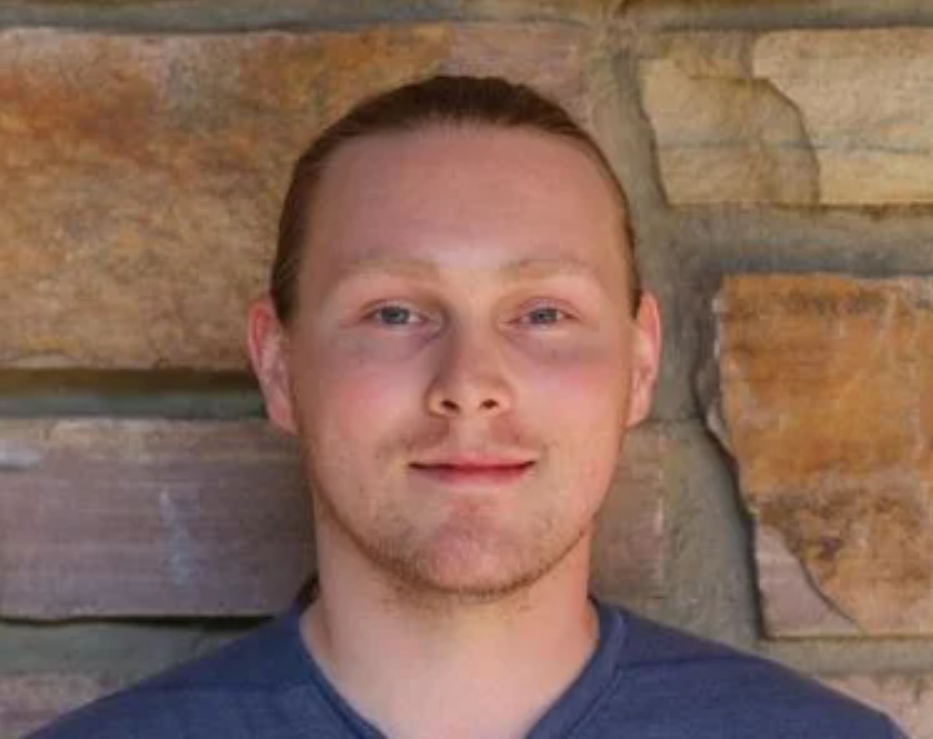
\includegraphics[height=\headshotsize, trim={3cm, 0cm, 3cm, 0cm}, clip=true]{headshot_sage}
\hspace{.5cm}
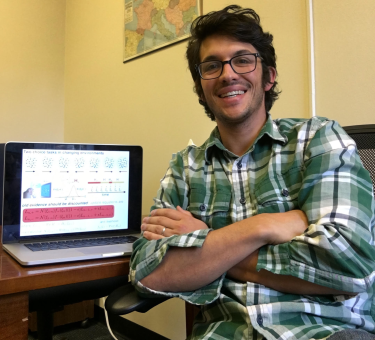
\includegraphics[height=\headshotsize, trim={5.1cm, 6cm, 2cm, 0cm}, clip=true]{headshot_zack}
\hspace{.5cm}
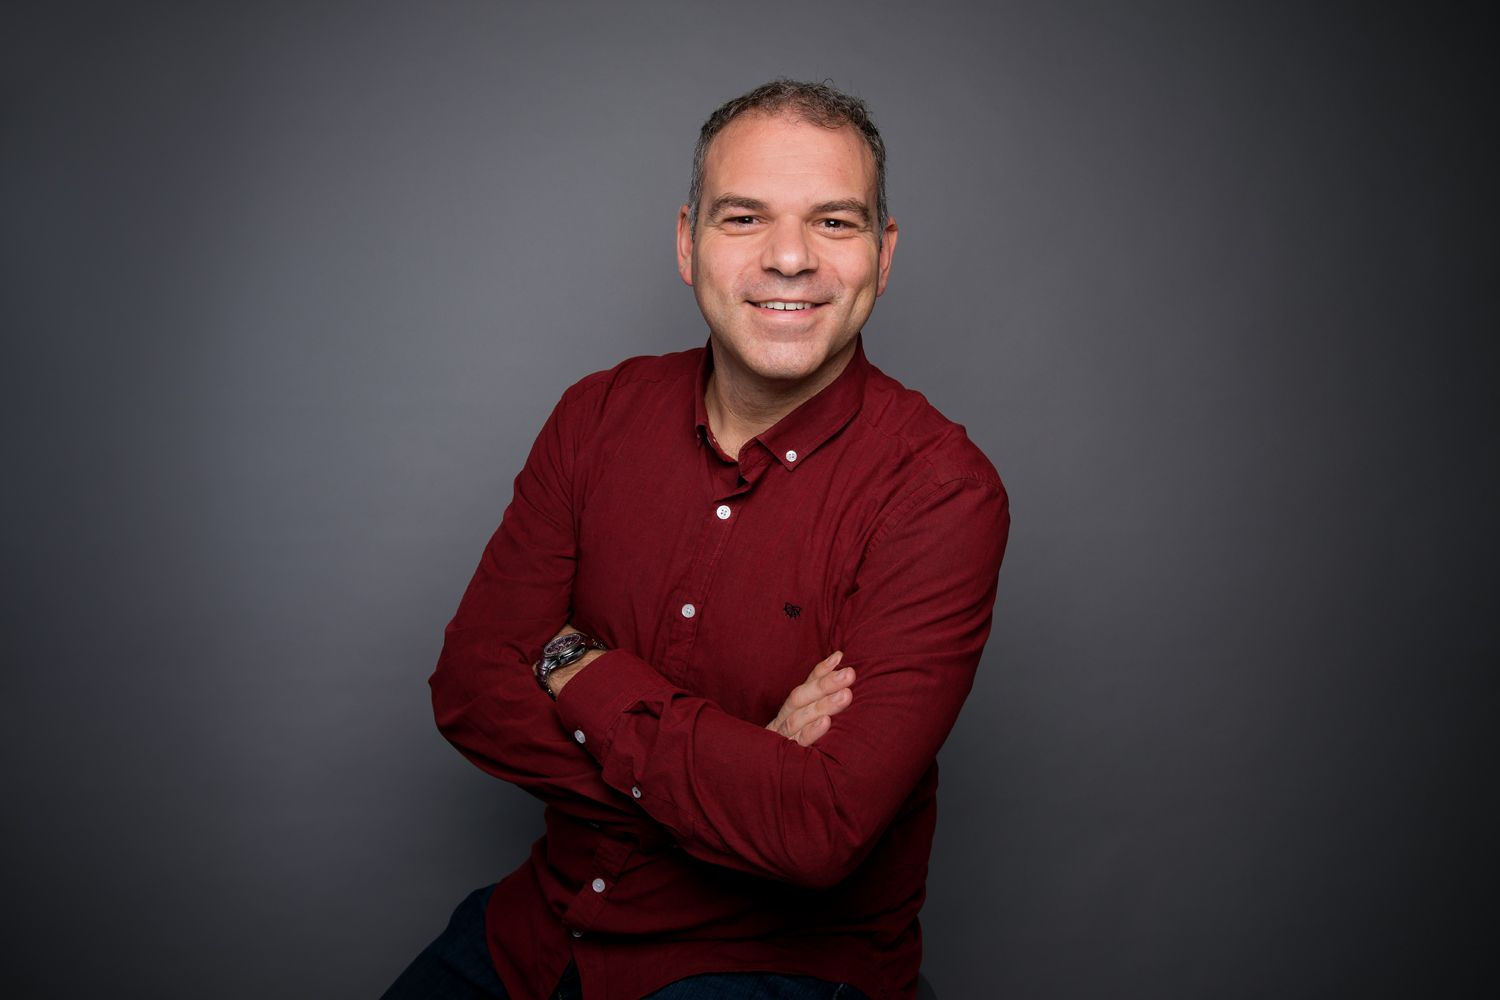
\includegraphics[height=\headshotsize, trim={21cm, 20cm, 18cm, 2cm}, clip=true]{headshot_daniele}
}
%%% Poster Content %%%

%%%%%%%%%%%%%%%%%%%
%%% Column 0
%%%%%%%%%%%%%%%%%%%
\headerbox{Summary}{name = summary, column = 0}{
	\textbf{Goal:} To create and test a neural field solver using radial basis function quadrature.
	The method should be
	\vspace{-1em}
	\begin{itemize}[leftmargin=*]
		\setlength\itemsep{-.5em}
		\item High-order accurate
		\item Stable
		\item Geometrically flexible
		\item Fast (low complexity)
	\end{itemize}

	In the future, we will extend this to realistic curved 2D spatial domains.
}

\headerbox{Neural Field Models}{name = neuralfield, column = 0, below=summary}{
	\begin{itemize}[leftmargin=*]
		\setlength\itemsep{-.5em}
		\item Tissue level models
		\item Integro-differential equation(s)
		\item Integral kernel represents neural network connectivity
		\item Non-linear firing rate function captures non-linear neural dynamics
	\end{itemize}
	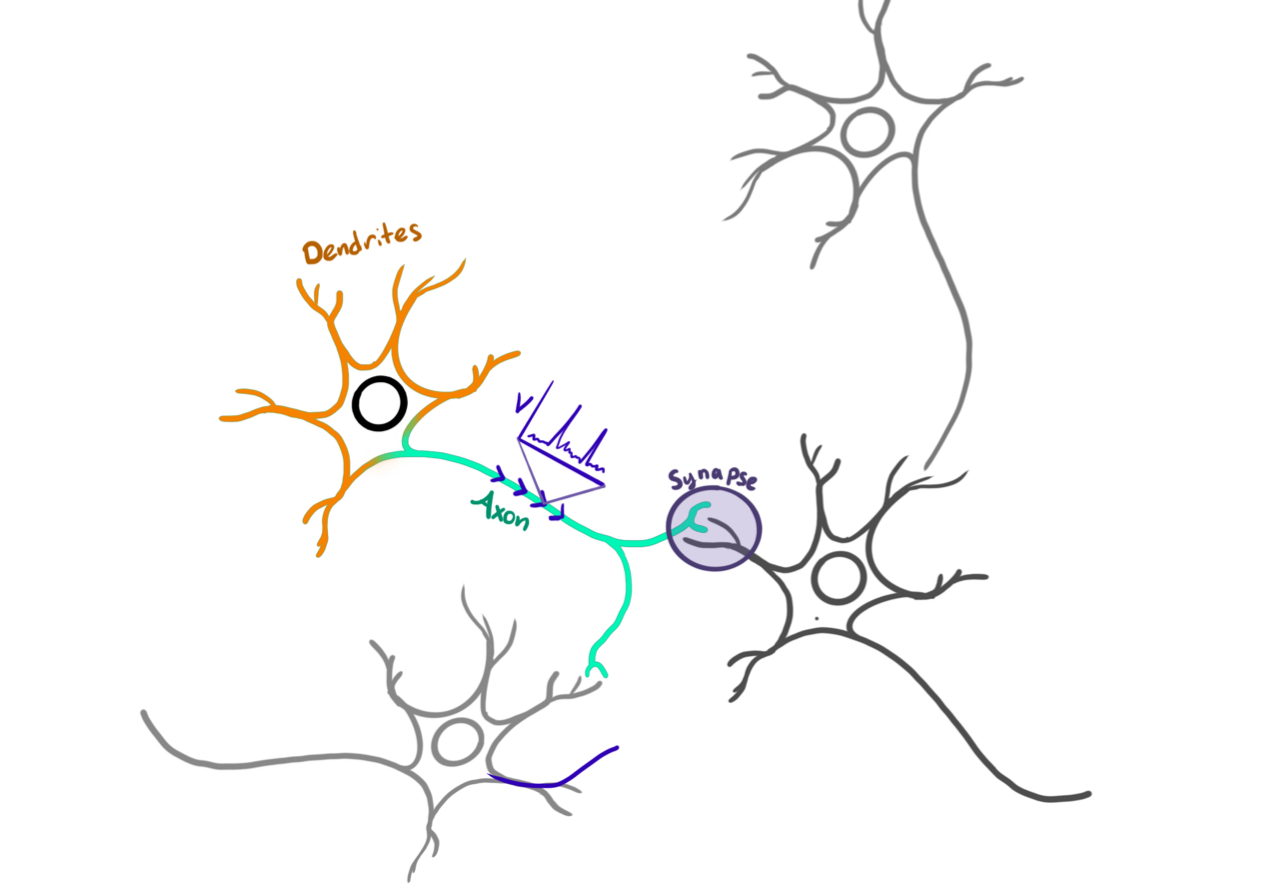
\includegraphics[width=\linewidth]{images/neurons}
	\centerline{Image by Heather Cihak.} \\

	$\partial_t u(t, \vecx) = -u + \iint_\Omega w(\vecx, \vecy) f[u(t, \vecy)] \ d\vecy$
	\begin{itemize}[leftmargin=*]
		\setlength\itemsep{-.5em}
		\item $u(t, \vecx)$ --- Neural activity
		\item $w(\vecx, \vecy)$ --- Connectivity kernel
		\item $f(\cdot)$ --- Non-linear firing rate function
		\item $\Omega = [0, 1]^2$ for now.
	\end{itemize}
}

%%%%%%%%%%%%%%%%%%%
%%% Column 1 
%%%%%%%%%%%%%%%%%%%
\headerbox{$\begin{array}{l}
\text{Radial Basis Function}\\ \text{Quadrature Formuale}
\end{array}$
}{name = rbfqf, column = 1, boxheaderheight=1.3cm}{
	% Itemize Example:
	\begin{itemize}[leftmargin=*]
		\setlength\itemsep{-.2em}
		\item Place $N$ nodes in $\Omega$
		\item Partition $\Omega$ into elements
		\item For each element
		\vspace{-1em}
		\begin{itemize}
			\setlength\itemsep{-.2em}
			\item select the $k$ nearest nodes \\(the stencil),
			\item interpolate Lagrange functions,
			\item integrate over the element,
			\item sum over interpolants
		\end{itemize}
		\setlength\itemsep{-1em}
		\item sum over elements
	\end{itemize}
	\vspace{-0.5em}
	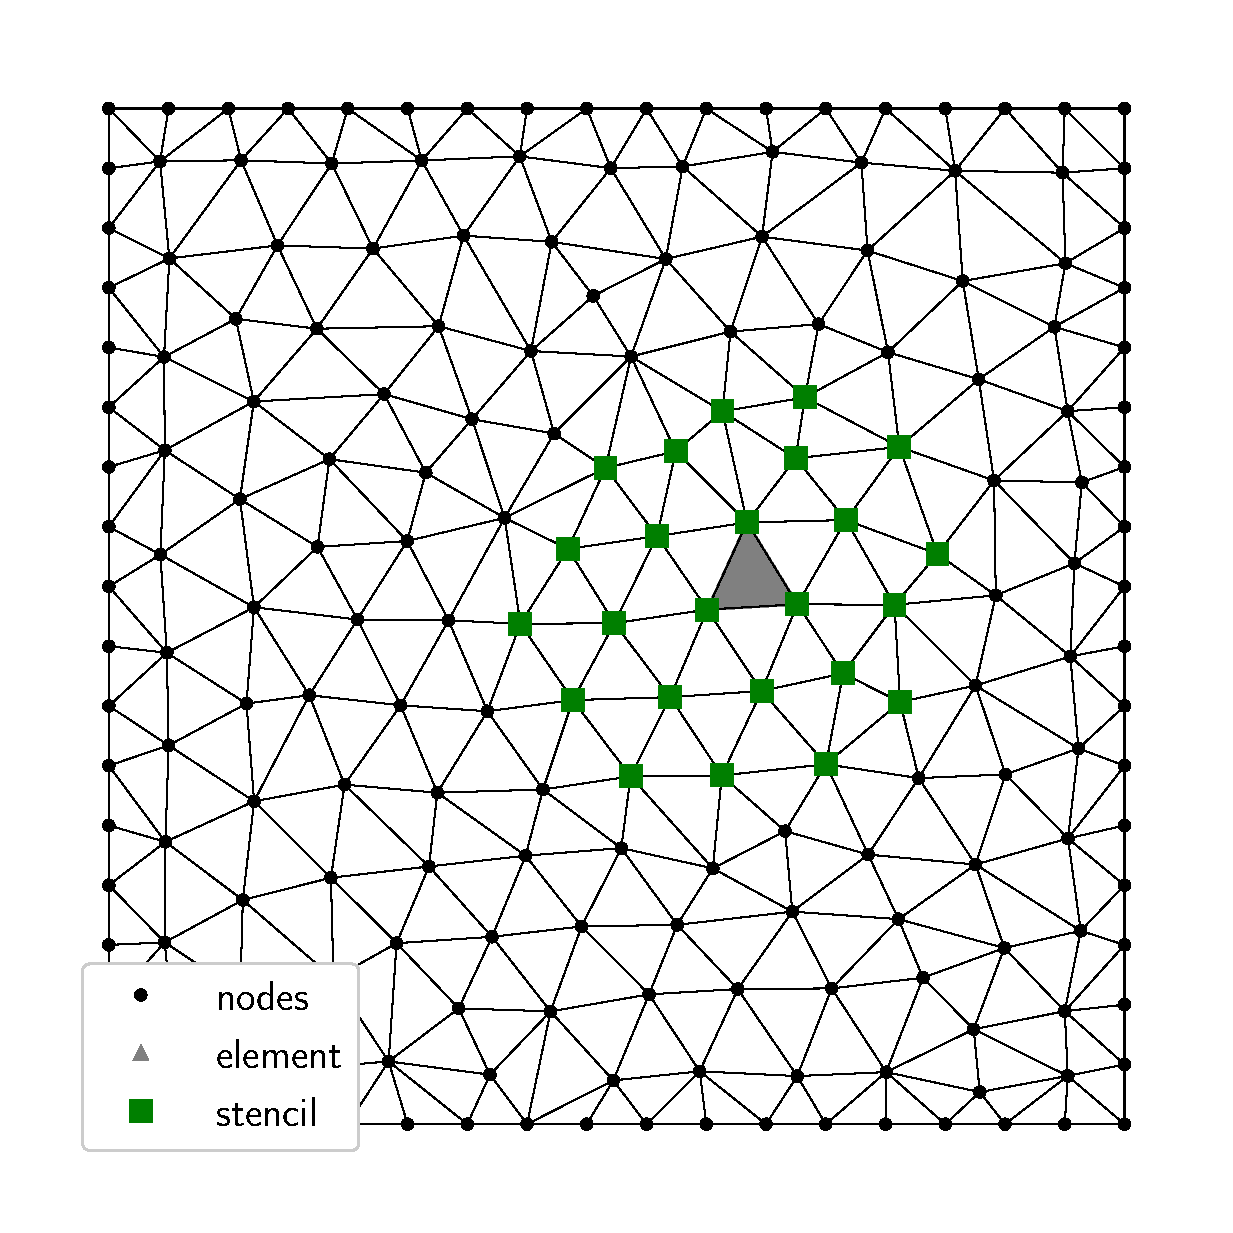
\includegraphics[width=\linewidth, trim={0cm, 1.1cm, 0cm, 1.4cm}, clip=true]{images/triangulation}
	The local interpolants have the form
	\vspace{-0.5em}
	\[
		s(\vecx) = \sum_{i=1}^k c_i \phi(\norm{\vecx - \vecx_i}) + \sum_{j=1}^m \gamma_i \pi_j(\vecx)
	\]
	\vspace{-2em}
	\begin{itemize}[leftmargin=*]
		\setlength\itemsep{-.2em}
		\item $\phi$ - radial basis function \\
		(eg. $\phi(r) = r^3$)
		\item $\{\pi_{j}\}_{j=1}^m$ - polynomial basis
		\item $k$ interpolation conditions
		\item $m$ moment conditions
	\end{itemize}
	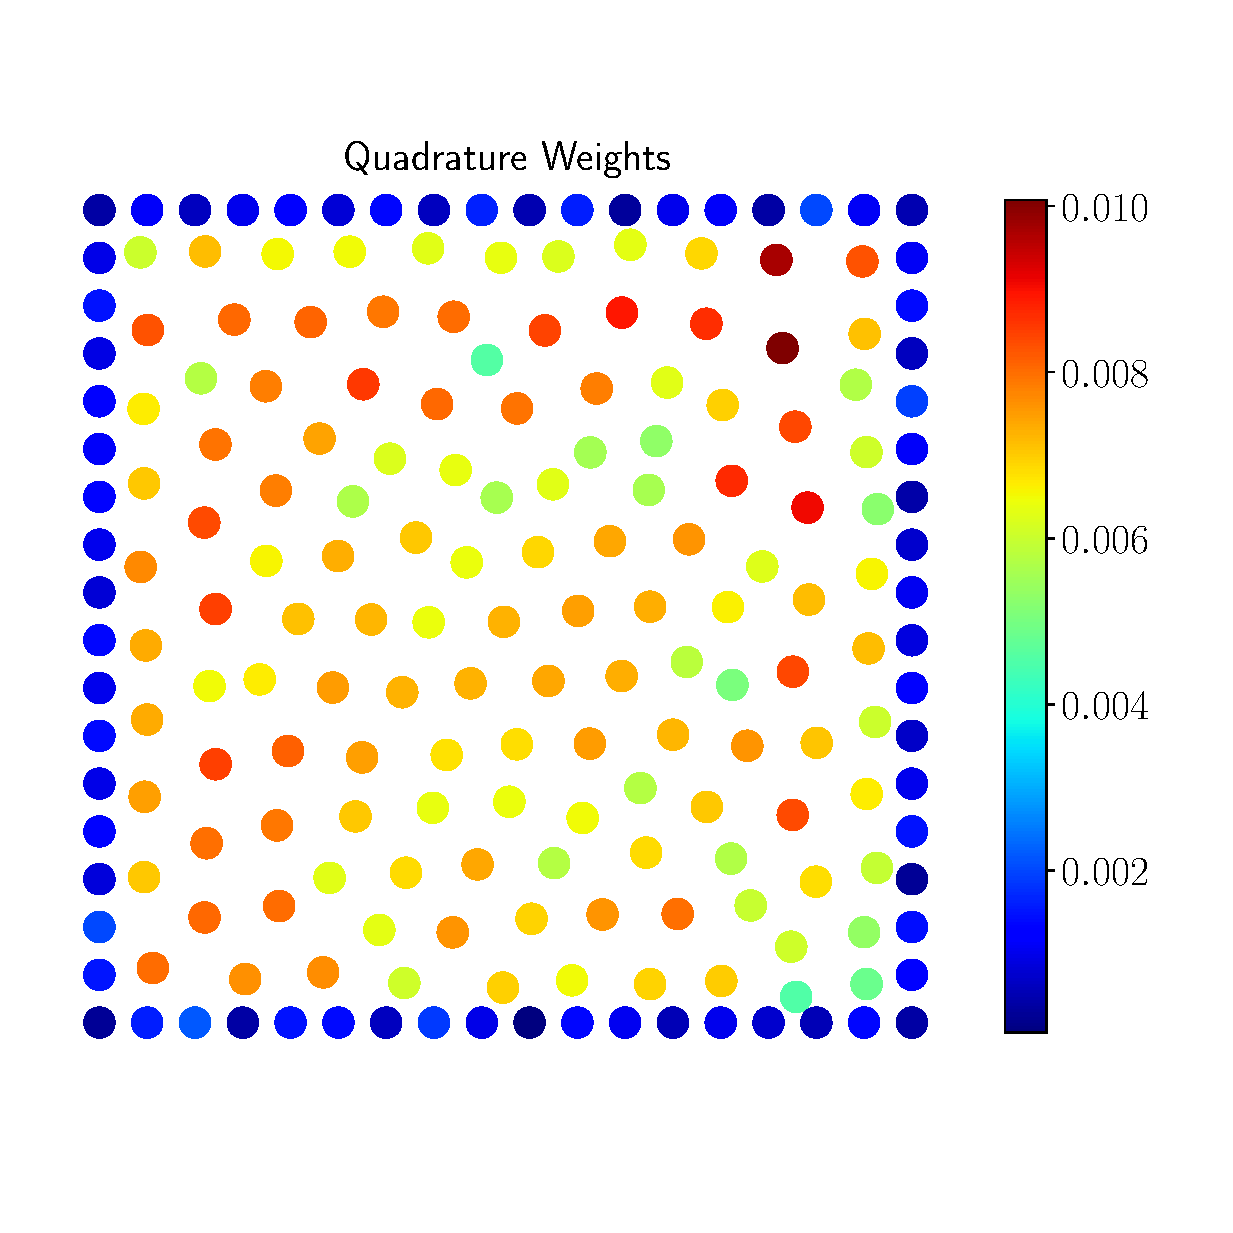
\includegraphics[width=\linewidth, trim={0cm, 3cm, 0cm, 2cm}, clip=true]{images/weights}
	\vspace{-.3cm}
}

%%%%%%%%%%%%%%%%%%%
%%% Column 2
%%%%%%%%%%%%%%%%%%%
\headerbox{Quadrature Convergence}{name = quad_convergence, column = 2}{
	\begin{itemize}[leftmargin=*]
		\setlength\itemsep{-.2em}
		\item No proven convergence rate.
		\item We expect at least $\mathcal{O}(d+1)$, where $d$ is the degree of polynomial basis. (Think trapezoidal rule.)
		\item We test this on a product of Chebyshev polynomials.
	\end{itemize}
	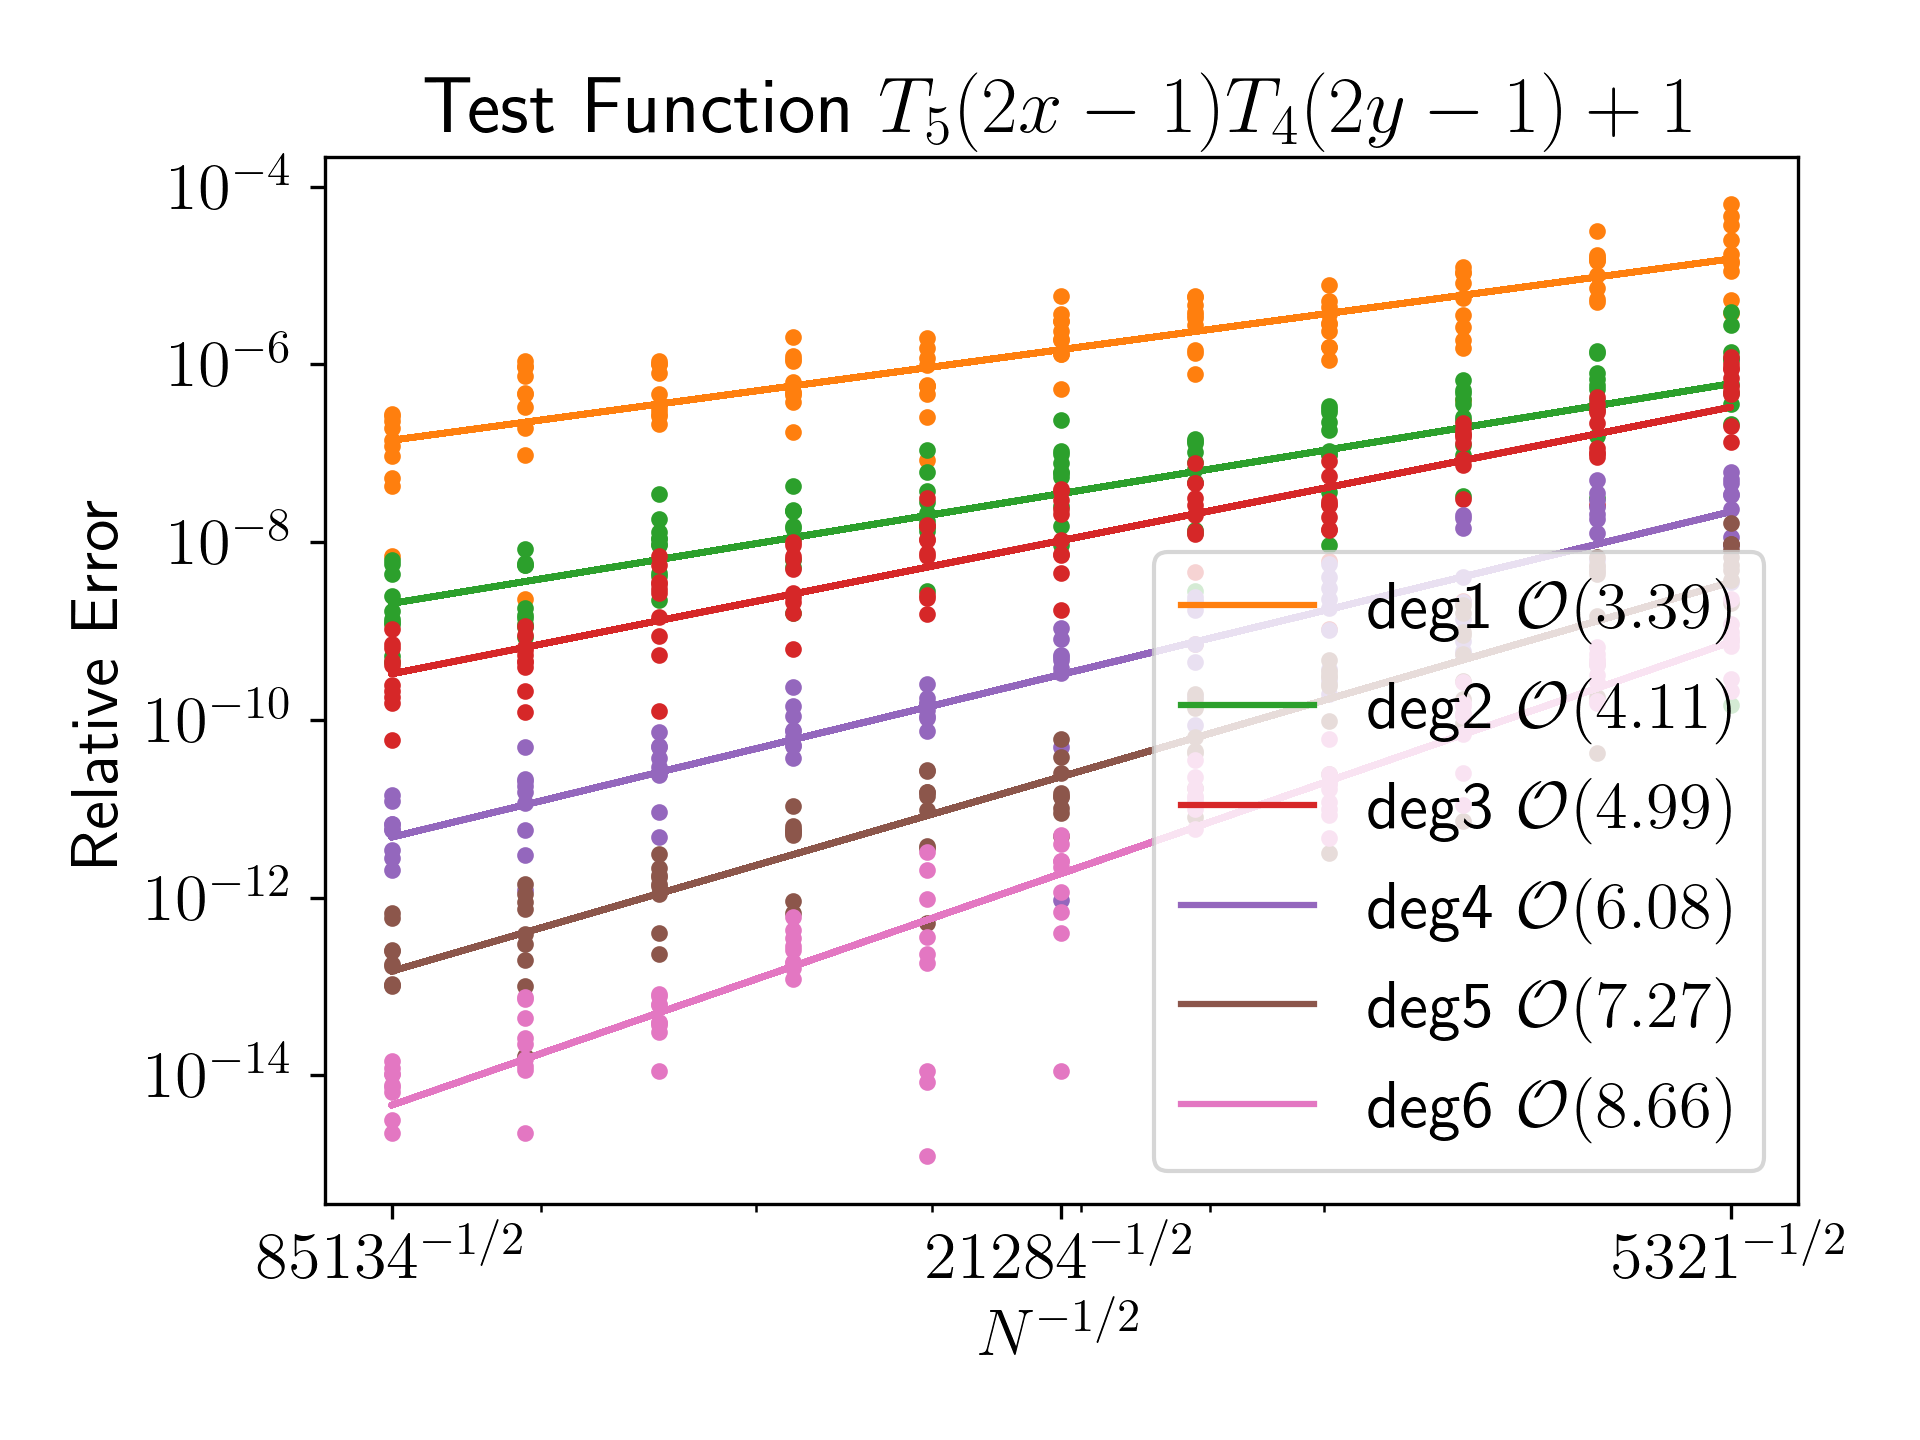
\includegraphics[width=0.95\linewidth]{images/quad_convergence}
}

\headerbox{Spatial Analysis}{name = quad, column = 2, below=quad_convergence}{
	\begin{itemize}[leftmargin=*]
		\setlength\itemsep{-.2em}
		\small
		\item Gaussian test functions centered at $(x_0, y_0)$
		\item Scattered Nodes vs Regular Hex Grid
		\item Error is continuous w.r.t. $(x_0, y_0)$
		\item Hex grid has spectral accuracy away from boundary
	\end{itemize}
	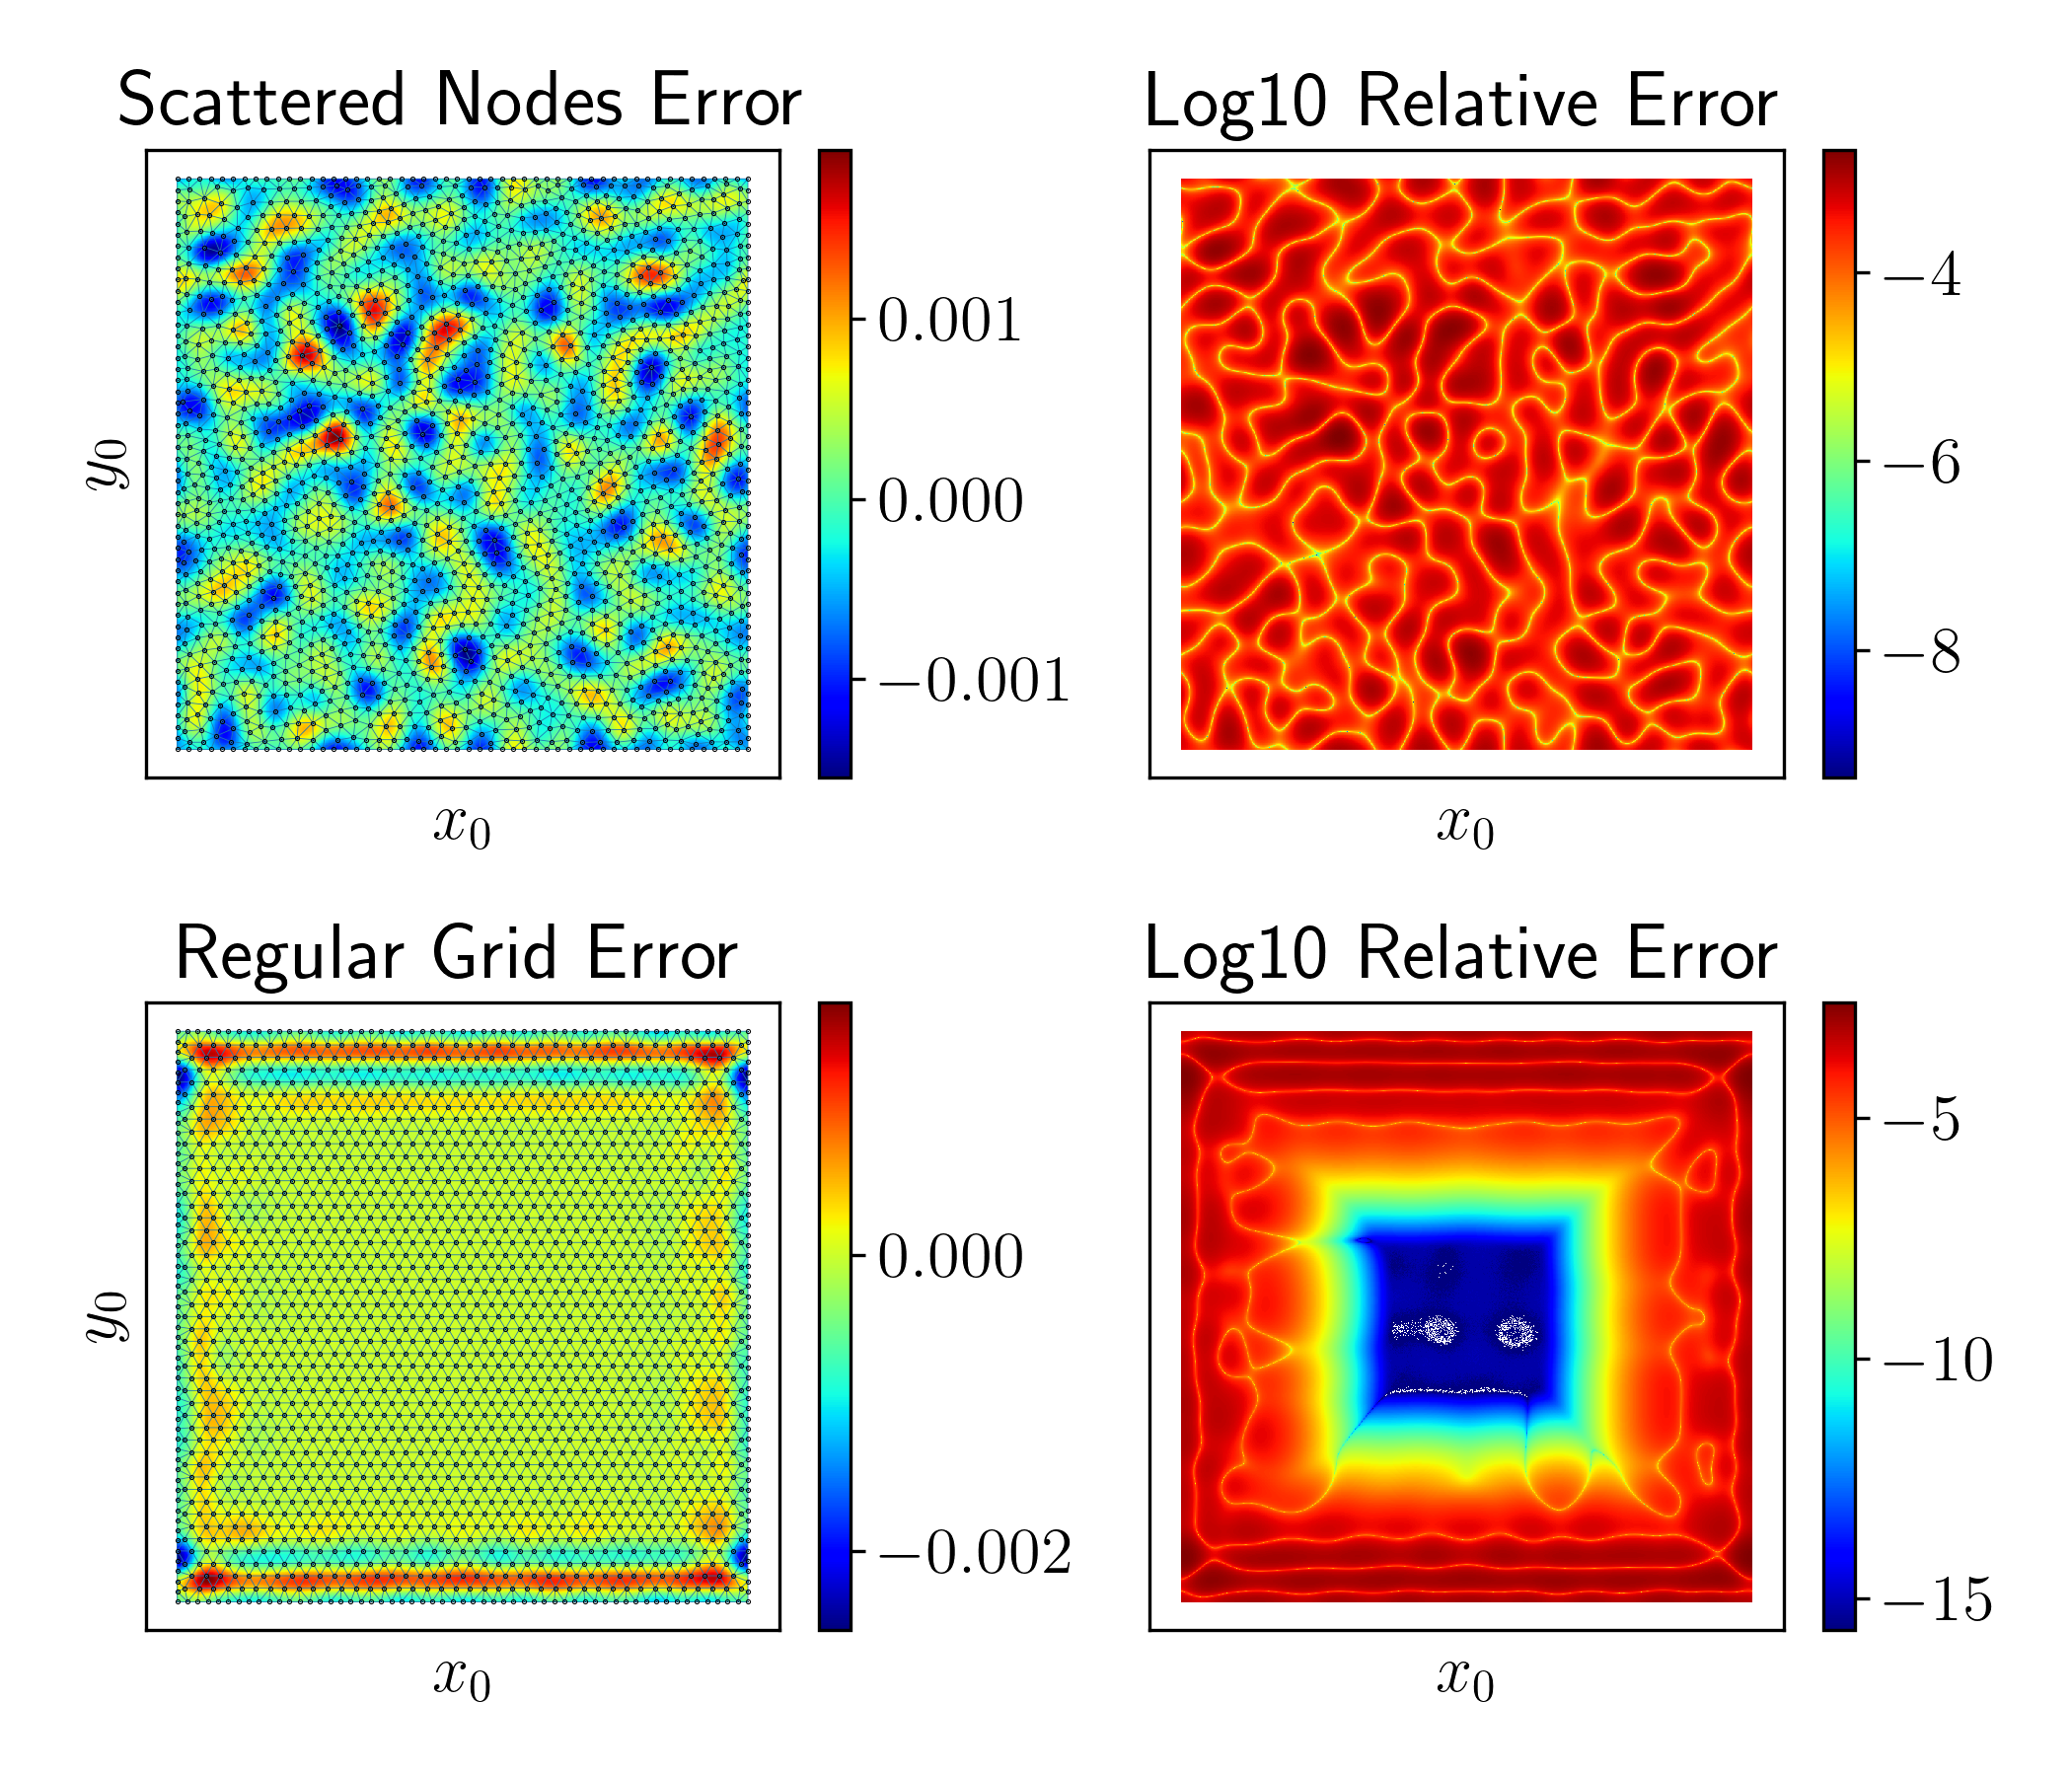
\includegraphics[width=\linewidth, trim={.5cm, .5cm, .5cm, 0cm}, clip=true]{images/poster_space_combined}
}

%%%%%%%%%%%%%%%%%%%
%%% Column 3
%%%%%%%%%%%%%%%%%%%
\headerbox{Next Steps}{name = ivp, column = 3}{
	\textbf{Projection Method}
	\begin{itemize}[leftmargin=*]
		\setlength\itemsep{-.2em}
		\small
		\item D. Avitable (2023)
		\item Framework for error analysis of neural field models
		\item Separates error into projection error and quadrature error
		\item We will unify these errors using RBF interpolation (projection) and RBF-QF.
	\end{itemize}
	\textbf{Curved 2D Manifolds}
	\begin{itemize}[leftmargin=*]
		\setlength\itemsep{-.2em}
		\small
		\item Reeger et al. (2016 \& 2018)
		\item Extended RBF-QF to 2D manifolds
		\item We will
	\end{itemize}
	\textbf{Corticol Spreading Depression}
	\begin{itemize}[leftmargin=*]
		\setlength\itemsep{-.2em}
		\small
		\item Reeger et al. (2016 \& 2018)
		\item Extended RBF-QF to 2D manifolds
		\item We will
	\end{itemize}
}

\headerbox{References and Funding}{name = ref, column = 3, below=ivp}{
	% Itemize Example:
	\begin{itemize}[leftmargin=*]
		\setlength\itemsep{-.4em}
		\small{
			\item Avitable (2023) SIAM J. Numer. Anal. % projection paper
			\item Regeer et al. (2016) Proc. Royal A % smooth surfaces without boundary
			\item Reeger \& Fornberg (2018) J. Comp. Phys. % smooth surfaces with boundary
		}
	\end{itemize}
	% Figure Example: 
	\small{This work is supported by\\ NSF DMS-2207700 \\ NIH BRAIN 1R01EB029847-01}
}

%%%%%%%%%%%%%%%%%%%%%%%%%%%%%%%%%%%%%%%%%%%%%
\end{poster}
\end{document}

